\section{Introduction} 
Understanding the decisions behind Machine Learning (ML) techniques is important for their adoption into new areas where an AI\textquotesingle s decisions have greater consequences. This need for interpretability has created the push for explainable AI (XAI) \cite{Karlo:xai}.

There are multiple approaches to XAI, one approach is the interpretable machine learning (IML) method of model extraction \cite{Bastani:modelExtarct}. Where traditional tree-based methods for model extraction and XAI suffer from limitations due to the greedy nature of tree construction, multi-objective genetic programming can balance the evolution of accurate and simple trees instead of constructing them in a top down greedy manner. These simple extracted models can be interpreted by humans to gain insight into a black-box's predictions. That is applicable to any black-box (arbitrarily complex) classifier.


\section{The New Method}
%In this section, a novel tree-based method is proposed for XAI.
We use NSGA-II \cite{Deb:nsga2}, paired with strongly-typed GP (STGP) \cite{Montana:stgp}, to evolve decision tree-like structures, which simultaneously balance the complexity and the accuracy of the trees. Our goal is to outperform greedy methods, while still being computationally feasible. Another benefit of this approach is that a Pareto front of non-dominated trees is produced instead of just a single tree. This is useful for XAI as it allows a user to select a tree for visualisation at a desired complexity to accuracy trade-off point along the front.
\subsection{Overall Algorithm}
The overall training algorithm is shown in figure \ref{fig:evolution}. The black-box classifier is trained once only on the original data (x and y values), then the evolutionary process is performed based on the resulting predictions (\^{y}) from this black-box model. The evolutionary algorithm never sees the original labels (y), as this is instead attempting to recreate the predicted labels (\^{y}). At the end of the evolutionary run, the result is a set of Pareto optimal models/trees which approximate the complex black-box model. Only the model with the highest reconstructive ability is used here. The overall evolutionary process is similar to NSGA-II. When selecting individuals, the non-dominated sorting in NSGA-II algorithm is used to rank the individuals.
\subsubsection{Objective Functions}
\begin{itemize}
\item \textbf{Reconstruction ability} (\textit{maximisation}): The average weighted f1 metric as result of an internal (training set only) 3-fold (k=3) cross-validation on the tree
\end{itemize}
\begin{itemize}
\item \textbf{Complexity} (\textit{minimisation}): Number of splitting points (nodes) in the tree
\end{itemize}

\begin{figure}
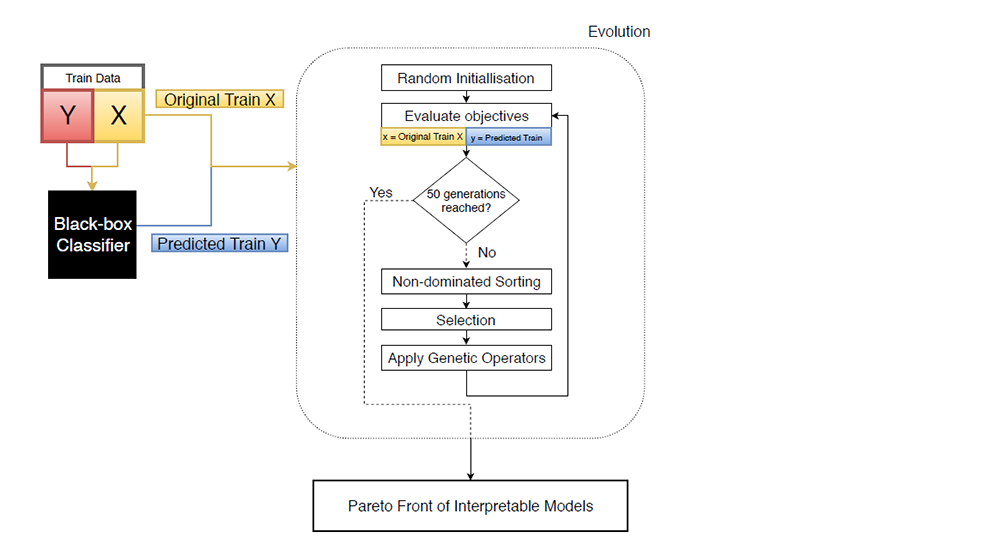
\includegraphics[width=0.75\textwidth]{evolution_process}
\caption{Evolutionary Training Process.}
\label{fig:evolution}
\end{figure}

\subsubsection{Representation}
The evolved trees are decision tree-like, meaning the input is at the root, the output at a leaf, and the internal nodes are splitting points. Traditionally with GP (parse-trees), the inputs are at the leaves, the output is at the root, and the internal nodes are functional components. To get around this, data is passed in at the leaves but only functions are returned until the root node, and then the functions are executed once we are at the root. For visualisation and use-cases, the two can be treated uniformly. 

Some simple patterns have needlessly complex representations in decision trees with axis-parallel splits. To solve this, the trees can construct features (as mathematical expressions) implicitly and check if those constructed features are greater than or equal to zero. Using constructed features is beneficial to XAI because simpler rules are learnt.
\section{Experiments}
\subsection{Experiment Details}
\subsubsection{Datasets}
A broad range of 30 datasets from the OpenML repository \cite{Van:openml} were used for comparison. The datasets were restricted to less than 15000 instances, less than 5 classes, and no missing values.
\subsubsection{Comparison Methods}
Current state-of-the-art approaches to model extraction were trialled:
\begin{itemize}
\item Bayesian rule lists (as pysbrl on pip)
\item A (h2o) decision tree
\item A simplified (scikit-learn) decision tree
\item Logistic regression with L1-regularization (from scikit-learn)
\end{itemize}
Pre-Processing: One-hot-encoding was required for the scikit-learn methods to support categorical features. Multi-interval discretization is applied for the Bayesian rule lists to support continuous features.
\subsubsection{GP Parameter Settings}
The evolutionary search was run for 50 generations, with 100 trees in each generation. Trees were limited to a maximum height of 17. A crossover rate of 0.8 was used, and a mutation rate of 0.2. Top performing individuals are never lost, as the $\mu + \lambda$ algorithm \cite{Beyer:evo_strat} is used, with both values set to the population size.
\subsubsection{Evaluation Measures}
\paragraph{Classification Performance}
For measuring performance, we use a weighted f1-measure scaled to the range 0\ldots100.
\paragraph{Complexity}
We define complexity as the number of splitting points in the tree. Constructed features count as multiple splits (f1+f2<=0 would count as 2). For Bayesian rule lists the complexity is measured as the number of rules + the number conjunctions in these rules. For logistic regression complexity is measured as the number of non-zero coefficients.
\subsubsection{Black-box Methods}
We chose three high performing black-box models, all implemented in h2o: Random Forests, Gradient Boosting (both with 500 trees) and a deep neural network (200 hidden layers with 200 neurons each).

\subsubsection{Significance Tests}
To compute whether the difference in reconstruction ability across datasets for each method was statistically significant, we used Friedman tests paired with Nemenyi post-hoc analysis. 

To show the average reconstruction ability for each method we present the average accuracy of a 10-fold cross-validation, where each method gets the same train-test sets. The averages are also across the 3 black-box methods therefore for each method, 30 runs are executed for each of the 20 datasets.
\subsection{Results}
We compare methods based on the number of times each method was dominated. For our method we select a single solution from our resultant frontier with the highest reconstruction ability to represent our methods performance. Where domination is defined as another method achieves a simpler representation with the same (or improved) recreation ability. GP (the proposed method) was not dominated on any of the datasets (Fig. \ref{fig:results}). \footnote{One caveat is that analysing the dominated counts alone is not a comprehensive indicator of performance, since both the simplest possible model (majority class) and the black-box model itself would never be dominated.} The resulting p-values from the significance tests are visualised in Fig. \ref{fig:results}.
%Another argument is that since GP was the only method which simultaneously balanced these objectives, the measure can be seen as biased towards the proposed method. This is true, but also shows the usefulness of population-based techniques such as GP as they can effectively optimise multiple objectives simultaneously. This shows that multi-objective optimisation is a good choice for IML, as the objectives were optimised better than the existing approaches (in terms of dominance).
%


%Two figures put into one image to fit available space%
\begin{center}
\begin{figure}[h]
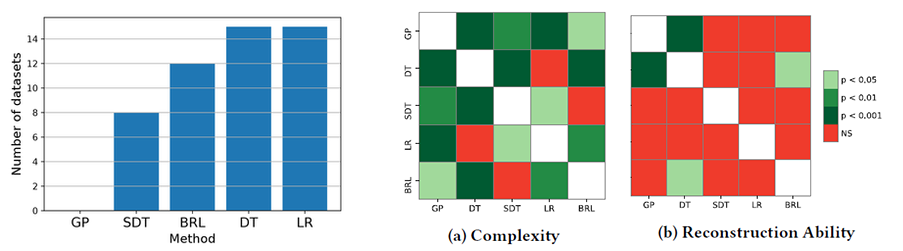
\includegraphics[width=\columnwidth]{results}
\caption{Method domination count (left) alongside Statistical significance testing (right).}
\label{fig:results}
\end{figure}
\end{center}





